
\subsection{{Description}}

    {In the context of Problem Set 1, the pivotal role of the ALU component emerges in the initial design of the General Processor Unit (GPU). Within this design, the Finite State Machine (FSM) orchestrates an up-counting pattern, influencing the operation selector signal directed to the ALU core. Tasked with executing arithmetic and logical operations based on inputs A and B, along with a 16-bit control unit input, the ALU component relies on microcode from the control unit as the operation-selector signal, dictating operations on A and B.}

    {Despite the reception of a 16-bit microcode, the ALU implements only nine distinct operations, outlined in Table 1. The core's functionalities are integral in producing an 8-bit output, denoted as "Result," representing the outcomes of operations on A and B. This output is intended for display on two 7-segment displays or LEDs. During simulation, the ALU allows visualization of the bit-value format of the output, Result, in the waveform editor window. In the subsequent FPGA board implementation, the output is showcased on two 7-segment displays in hexadecimal format.}
    
    {To integrate the ALU into the final circuit design, encompassing completed components such as Registers, FSM, Decoder units, a new schematic design is initiated. This design incorporates two registers, one ALU Core (ALU), one FSM, one Decoder, and three 7-segment displays. Input ports A and B (8-bit), output port Result (8-bit), and the clock port are established. Component connections are facilitated using single and multi-bit data buses, adhering to the schematics outlined in this report.}
    
    {Upon completion of the integration, the final circuit design undergoes synthesis and simulation. The verification of the ALU's functionality, including waveforms, constitutes a crucial aspect presented to the TA as part of the final report submission. The ALU's role in the initial GPU design is pivotal, ensuring the execution of specified operations and the generation of desired outputs.}

    \subsubsection{{Inputs}}

        \begin{itemize}
            \item   {\textbf{A (8-bit)}: First input of 8 bits for arithmetic and logical operations.}
            \item   {\textbf{B (8-bit)}: Second 8-bit input for arithmetic and logical operations.}
            \item   {\textbf{Control Unit (16-bit)}: Microcode input from the control unit, functioning as the operation-selector signal.}
        \end{itemize}

    \subsubsection{{Outputs}}

        \begin{itemize}
            \item   {\textbf{Result (8-bit)}: Output representing the result of operations performed on inputs A and B.}
            \item   {\textbf{7-Segment Displays/LEDs}: Display output in hexadecimal format during FPGA board implementation.}
        \end{itemize}

    \subsubsection{{Purpose}}

        \begin{itemize}
            \item   {\textbf{A and B}: Serve as inputs for arithmetic and logical operations.}
            \item   {\textbf{Control Unit}: Determines the operation to be applied to inputs A and B.}
            \item   {\textbf{Result}: Represents the output of operations on A and B.}
            \item   {\textbf{7-Segment Displays/LEDs}: Display the output in hexadecimal format during FPGA board implementation.}
        \end{itemize}
    
    \subsubsection{{Timing Diagram}}

    \begin{figure}[H]
        \centering
        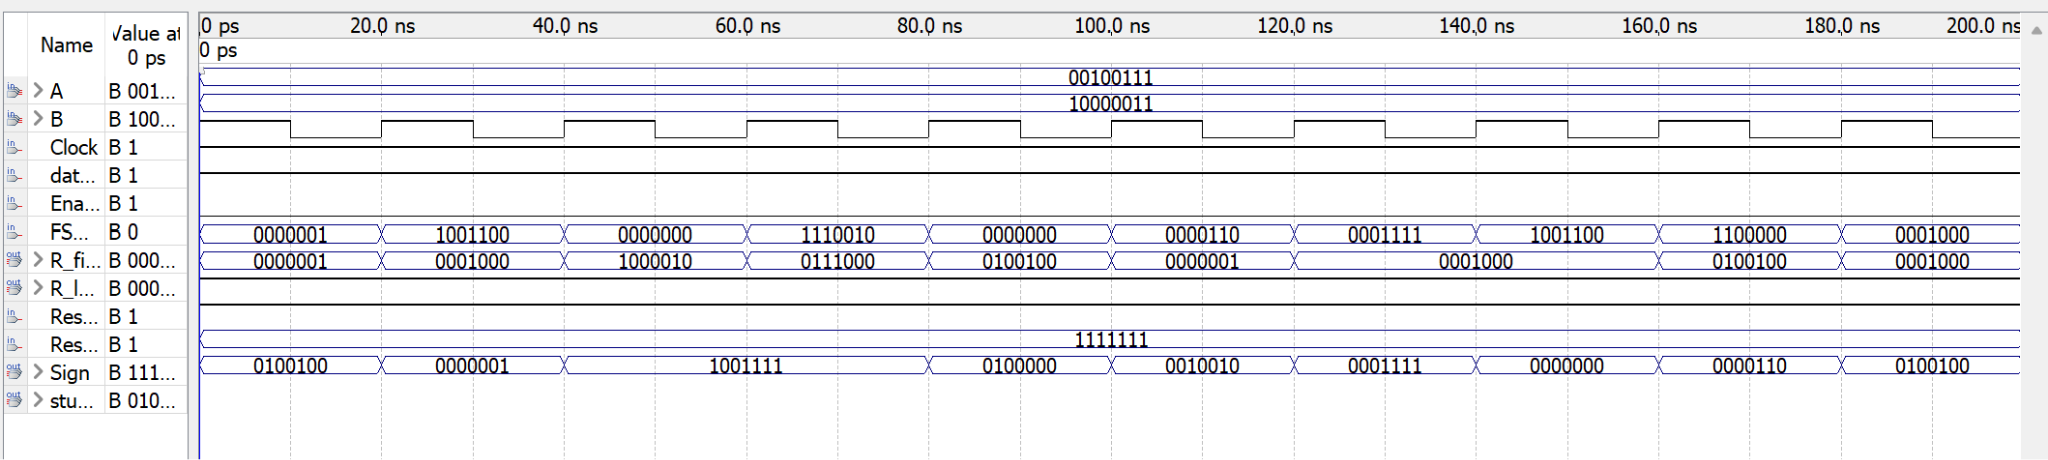
\includegraphics[width=15cm]{Pictures/ALU1WaveForm.png}
        \caption{{Timing Diagram of the Complete Logic Circuit 1}}
        \label{FSM}
    \end{figure}

    \subsubsection{{Block Diagram}}

        \begin{figure}[H]
            \centering
            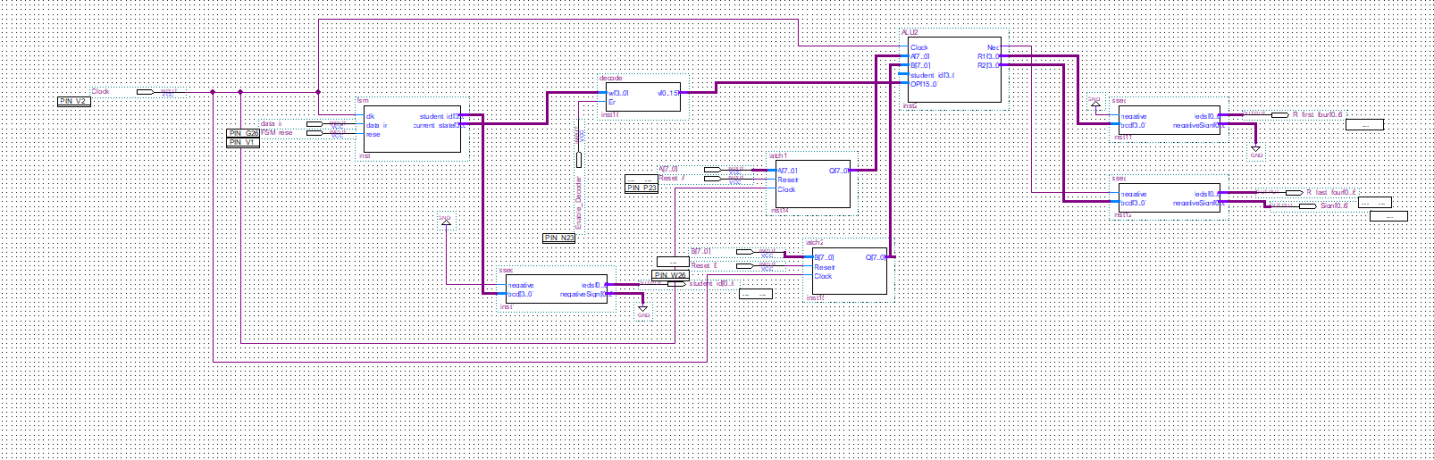
\includegraphics[width=15cm]{Pictures/P12BlockDia.png}
            \caption{{Block Diagram of the Complete Logic Circuit 1}}
            \label{FSM}
        \end{figure}

\subsection{{VHDL Code}}

    \subimport{./}{P1-VHDl}
